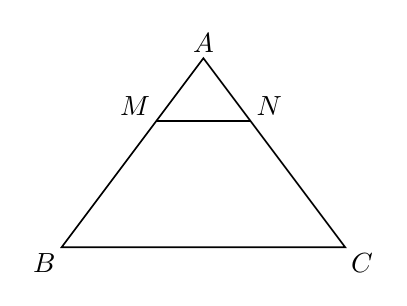
\begin{tikzpicture}[x=1cm,y=1cm,font=\normalsize,
 geometry edge/.style={solid,line width=.6pt},
 geometry mark/.style={solid,line width=.6pt},
 geometry label/.style={font=\normalsize,inner sep=2pt}]
\coordinate (A) at (0,2.4);
\coordinate (B) at (-1.8,0);
\coordinate (C) at (1.8,0);
\coordinate (M) at (-0.6,1.6);
\coordinate (N) at (0.6,1.6);
\draw[geometry edge] (A)--(B)--(C)--cycle;
\draw[geometry edge] (M)--(N);
\node[geometry label,above] at (A) {$A$};
\node[geometry label,below left] at (B) {$B$};
\node[geometry label,below right] at (C) {$C$};
\node[geometry label,above left] at (M) {$M$};
\node[geometry label,above right] at (N) {$N$};
\end{tikzpicture}
